\documentclass{article}
\usepackage[utf8]{inputenc}
\usepackage{subfigure}
\usepackage{geometry}
\usepackage{siunitx}
\usepackage{amsmath}

\geometry{
 a4paper,
 total={160mm,247mm},
 left=25mm,
 top=25mm,
 }

\title{Comp Astro Assignment 1}
\author{Cameron Smith }
\usepackage{natbib}
\usepackage{graphicx}

\begin{document}

\maketitle

\section*{Part 1}

While rk4 gives a good approximation of the ODE, it has no built-in way of
conserving necessary quantities such as angular momentum or energy. This results
in orbits such as the one in Figure \ref{fig:rk.1}, where the particle
gets closer and closer to the mass at the origin, speeding up as it goes, until
it's finally ejected altogether. This lack of conservation means that the errors
can build up, and both the angular momentum and total energy of the system
decrease over time, causing the orbit to decay (see Figures \ref{fig:rke}
and \ref{fig:rkL}). On the other hand, while the leapfrog scheme is only second
order, it is able to conserve angular momentum, and the error in the total
energy is symmetric, and does not increase over time, as can be seen
in Figures \ref{fig:lfL} and \ref{fig:lfe}. As a result, the orbit does not
decay over time, however does rotate if the timestep is too large, as can be
seen in Figures \ref{fig:lf.05} and \ref{fig:lf.1}.

\begin{figure}[h!]%
    \centering
    \subfigure[]{%
    \label{fig:lf.01}%
    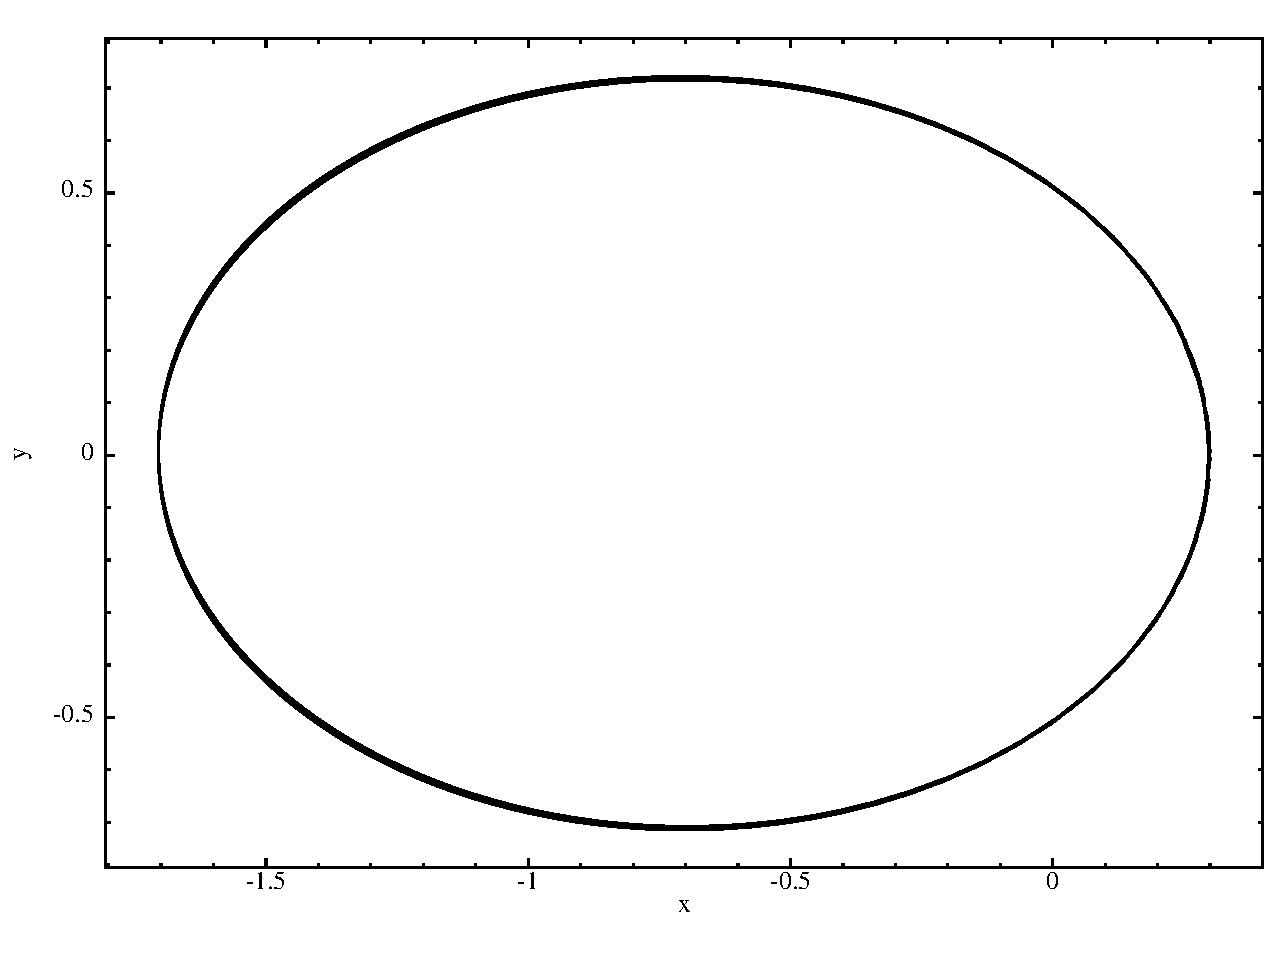
\includegraphics[height=2in]{leapfrog_0.01.pdf}}%
    \qquad
    \subfigure[]{%
    \label{fig:rk.01}%
    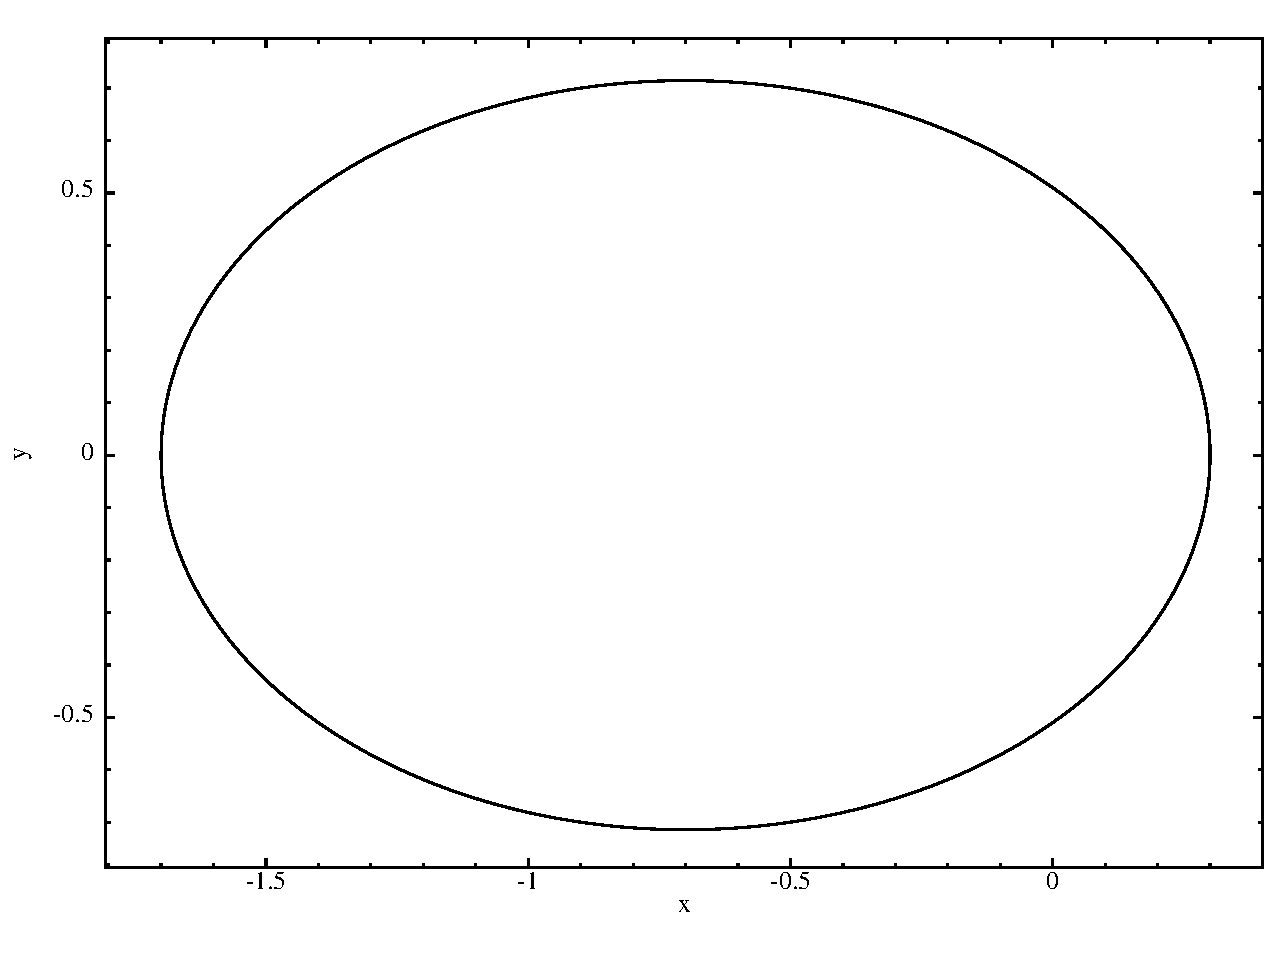
\includegraphics[height=2in]{rk40.01.pdf}}%
    \qquad
    \subfigure[]{%
    \label{fig:lf.05}%
    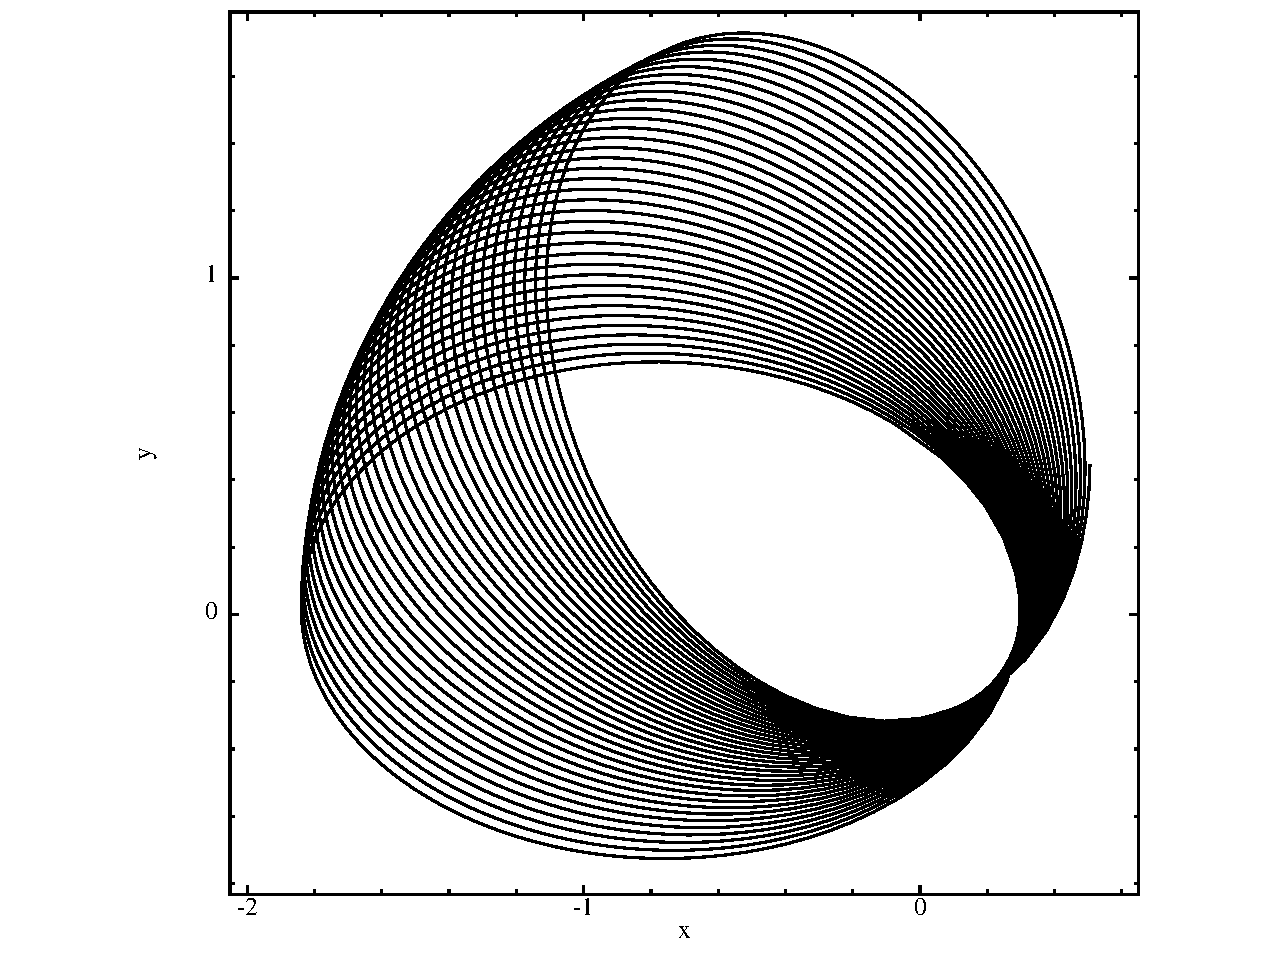
\includegraphics[height=2in]{leapfrog0.05.pdf}}%
    \qquad
    \subfigure[]{%
    \label{fig:rk.05}%
    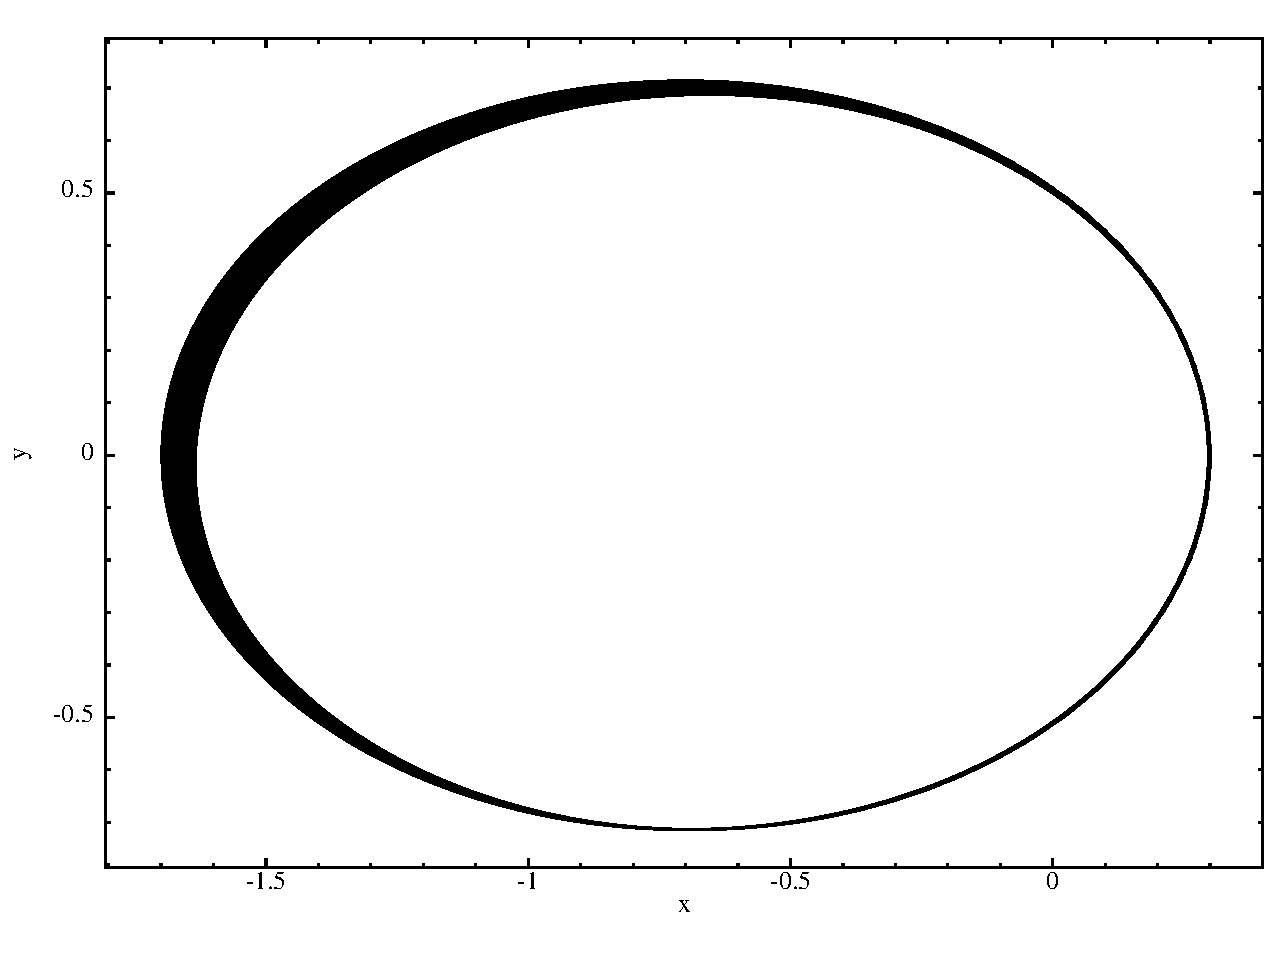
\includegraphics[height=2in]{rk40.05.pdf}}%
    \qquad
    \subfigure[]{%
    \label{fig:lf.1}%
    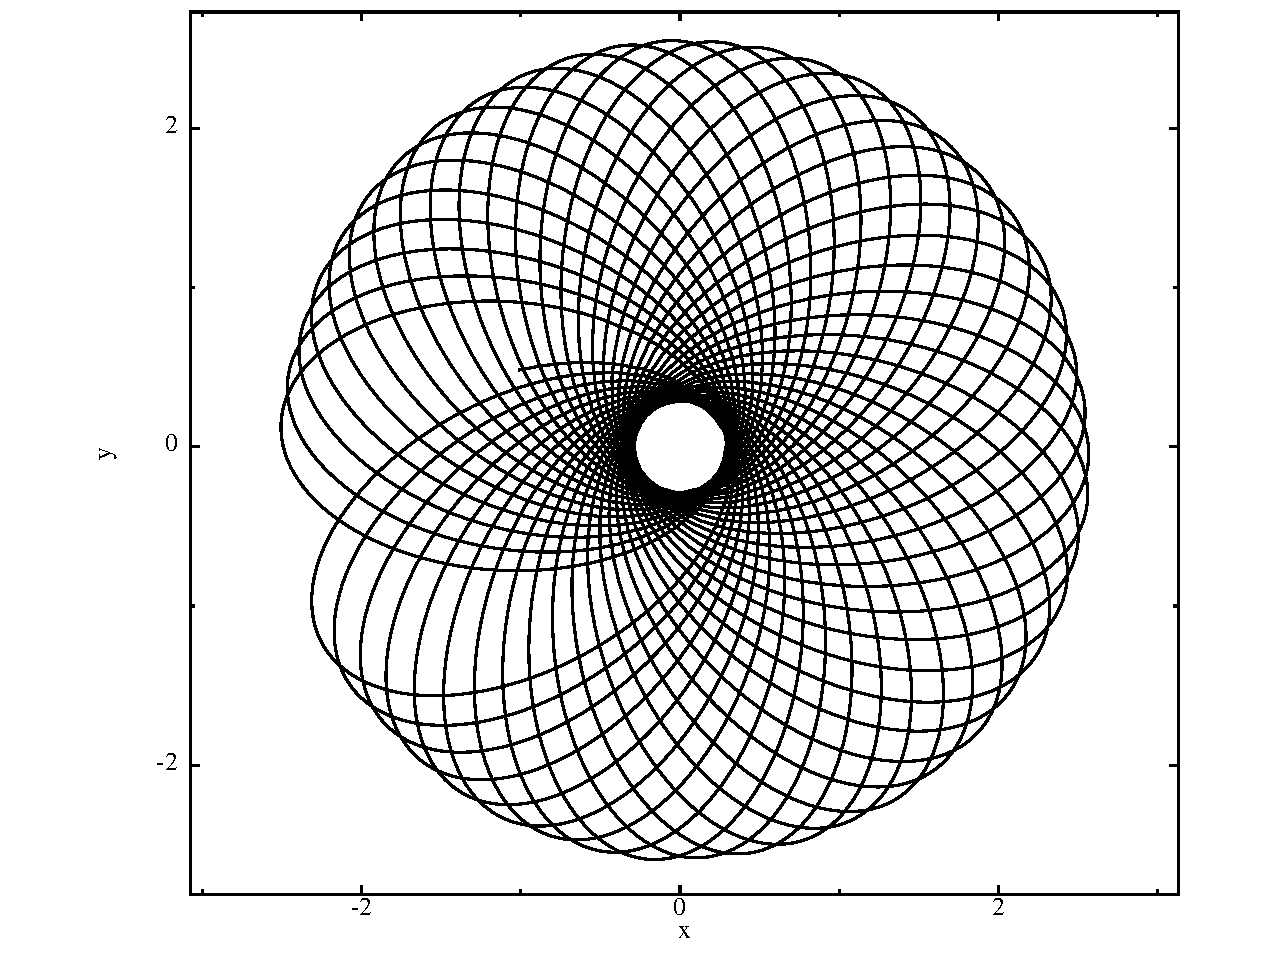
\includegraphics[height=2in]{leapfrog0.1.pdf}}%
    \qquad
    \subfigure[]{%
    \label{fig:rk.1}%
    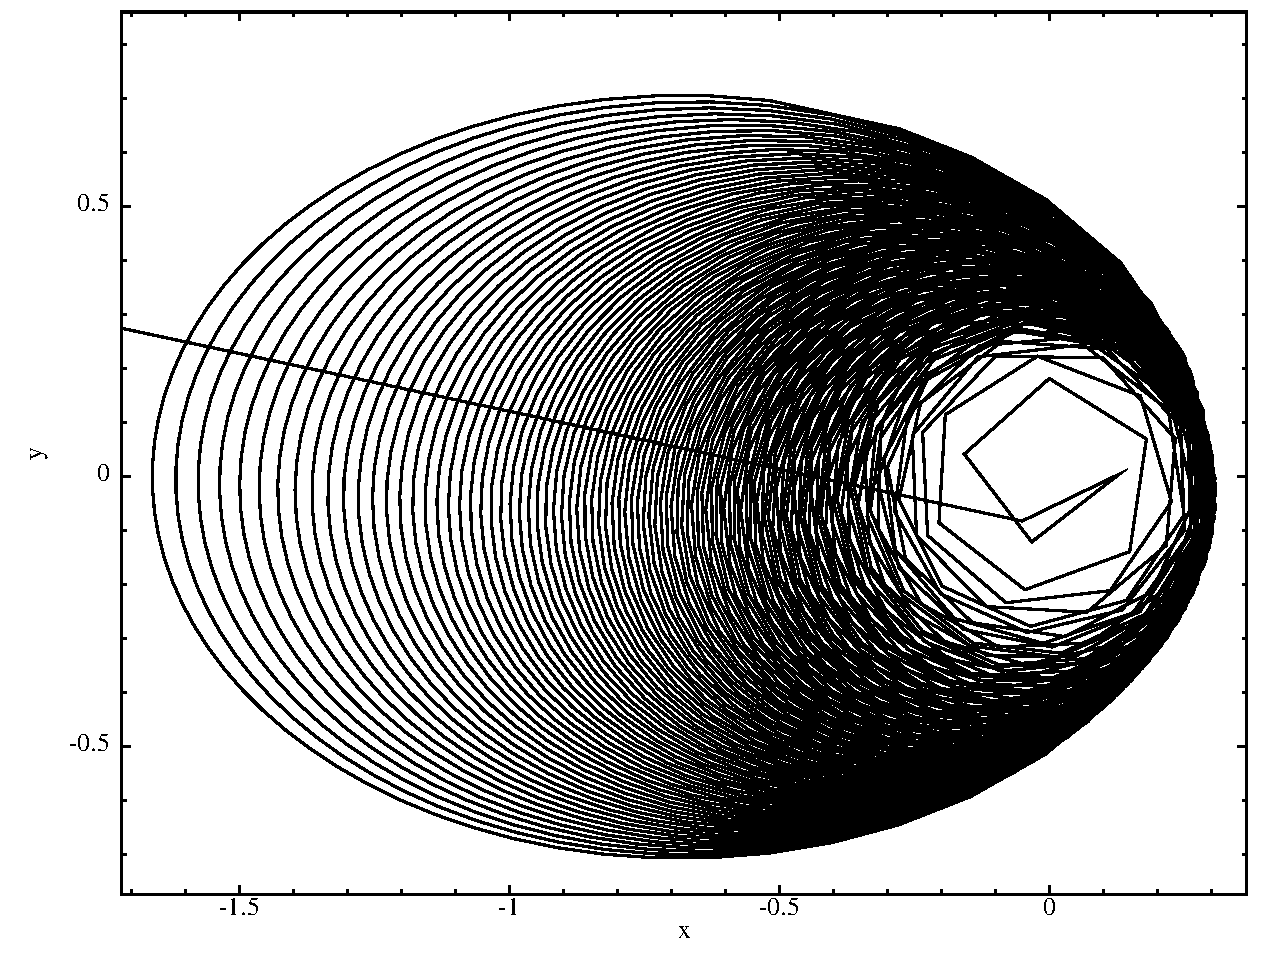
\includegraphics[height=2in]{rk40.1_close.pdf}}%
    \qquad
    \caption[]{Calculated orbits using the second order Leapfrog/Velocity Verlet
    scheme (left) and the forth order Runge-Kutta method (right), using time
    steps of $0.01$ (top) $0.05$ (middle) and $0.1$ (bottom).}.
\end{figure}


\begin{figure}[h!]%
    \centering
    \subfigure[]{%
    \label{fig:lfL}%
    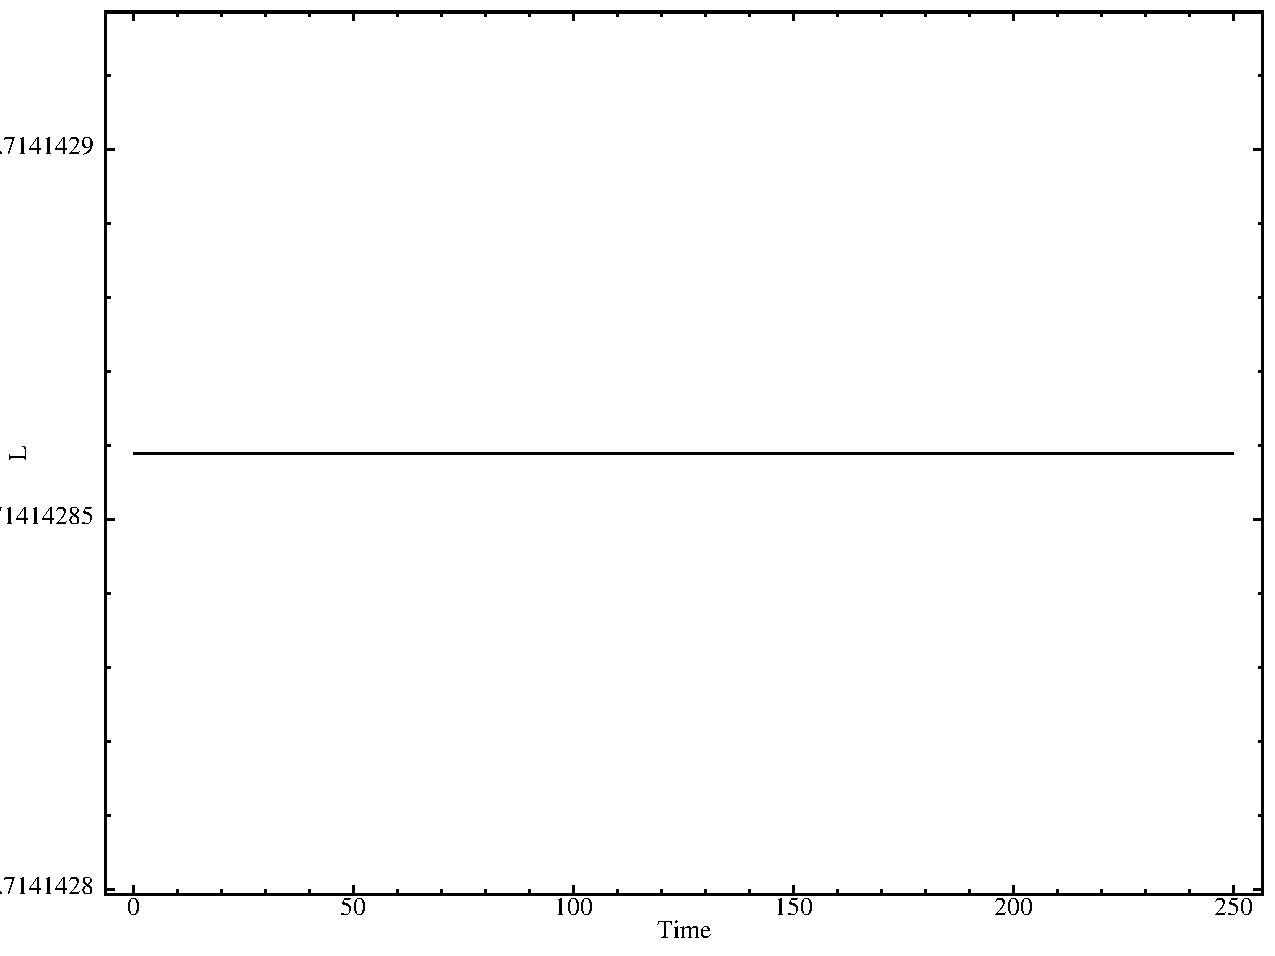
\includegraphics[height=2.2in]{leapfrogL.pdf}}%
    \qquad
    \subfigure[]{%
    \label{fig:rkL}%
    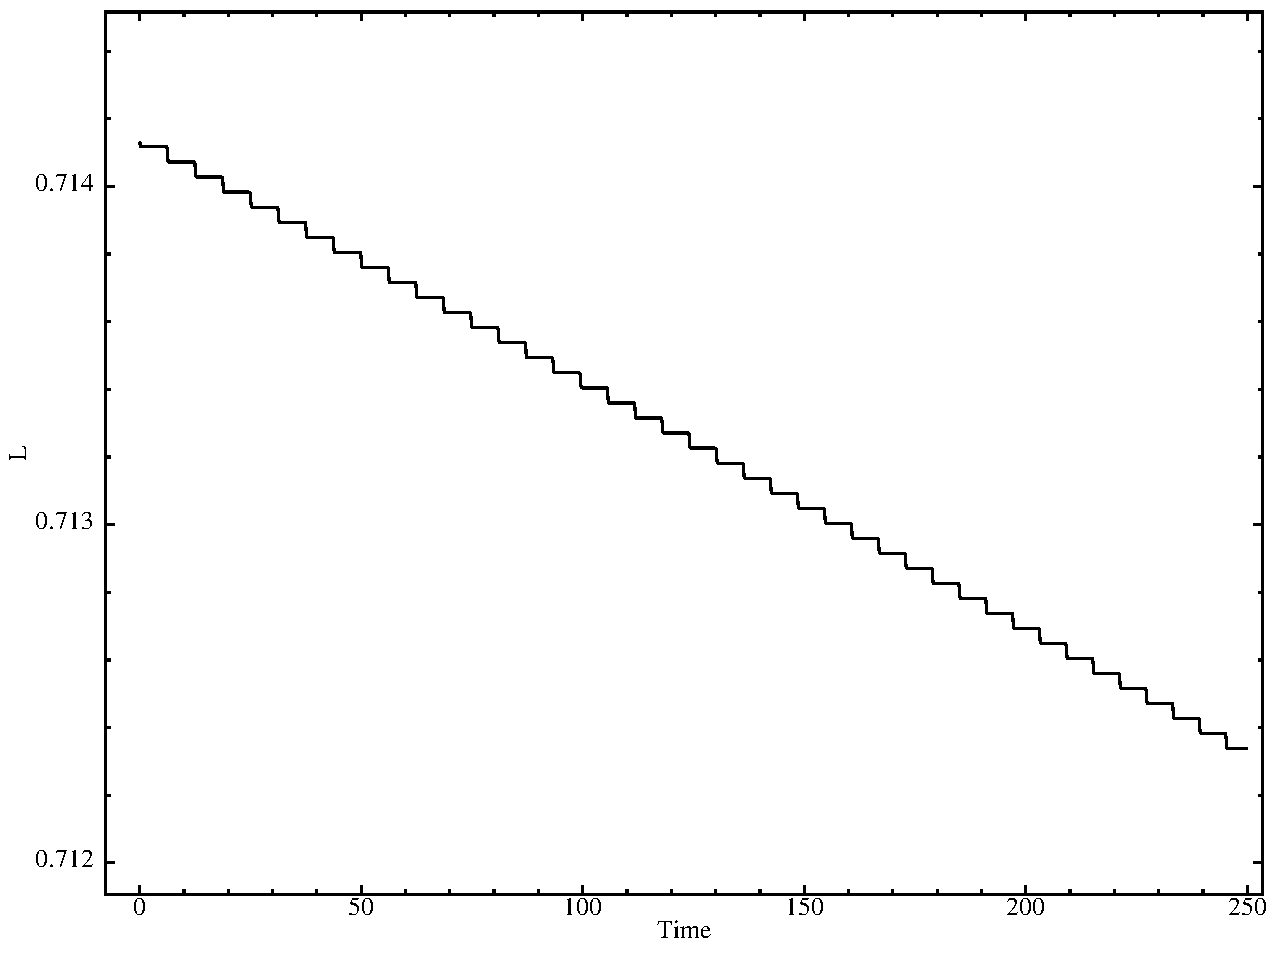
\includegraphics[height=2.2in]{rk40L.pdf}}%
    \qquad
    \subfigure[]{%
    \label{fig:lfe}%
    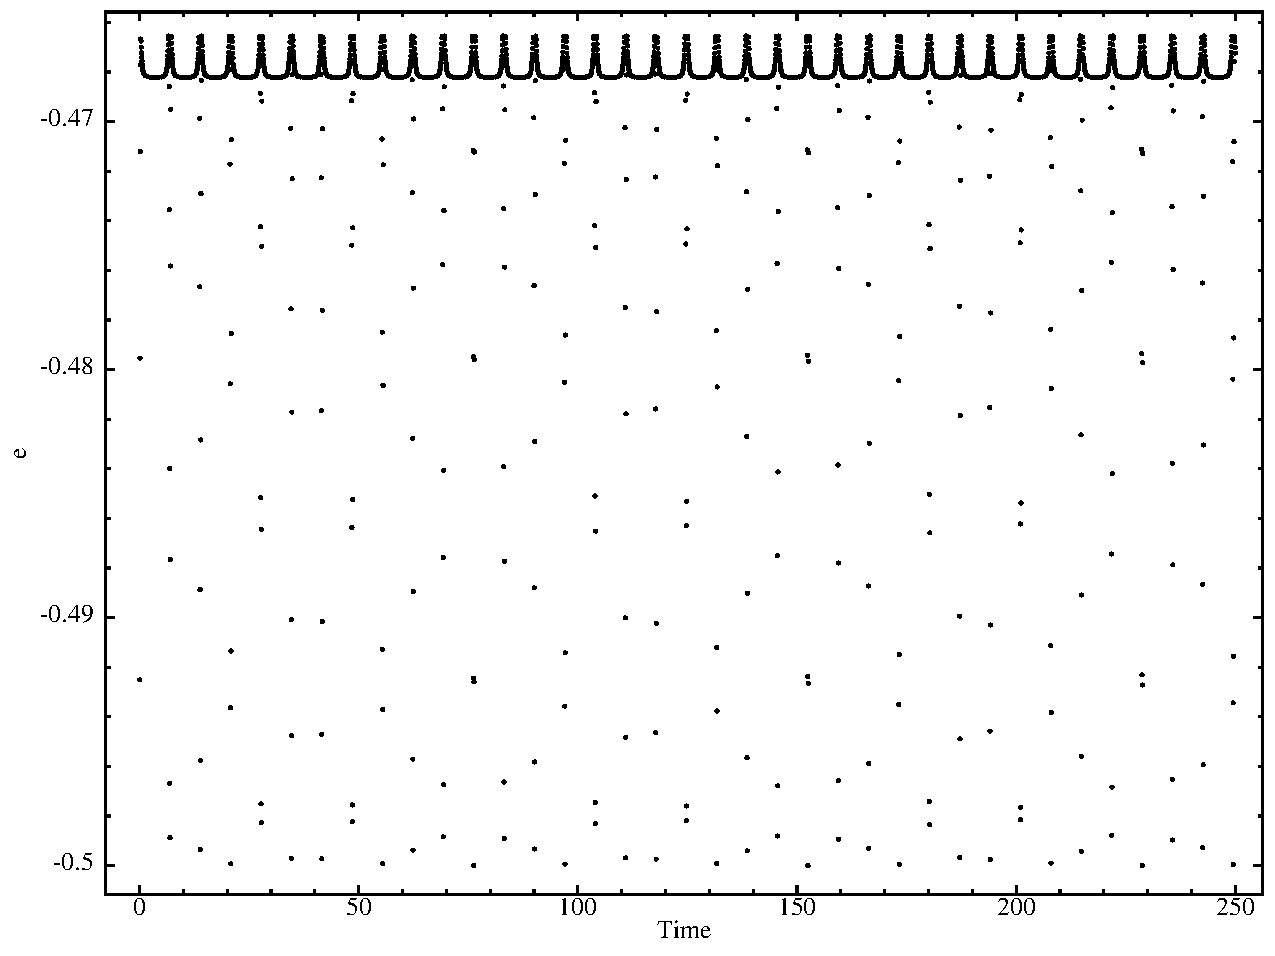
\includegraphics[height=2.2in]{leapfroge.pdf}}%
    \qquad
    \subfigure[]{%
    \label{fig:rke}%
    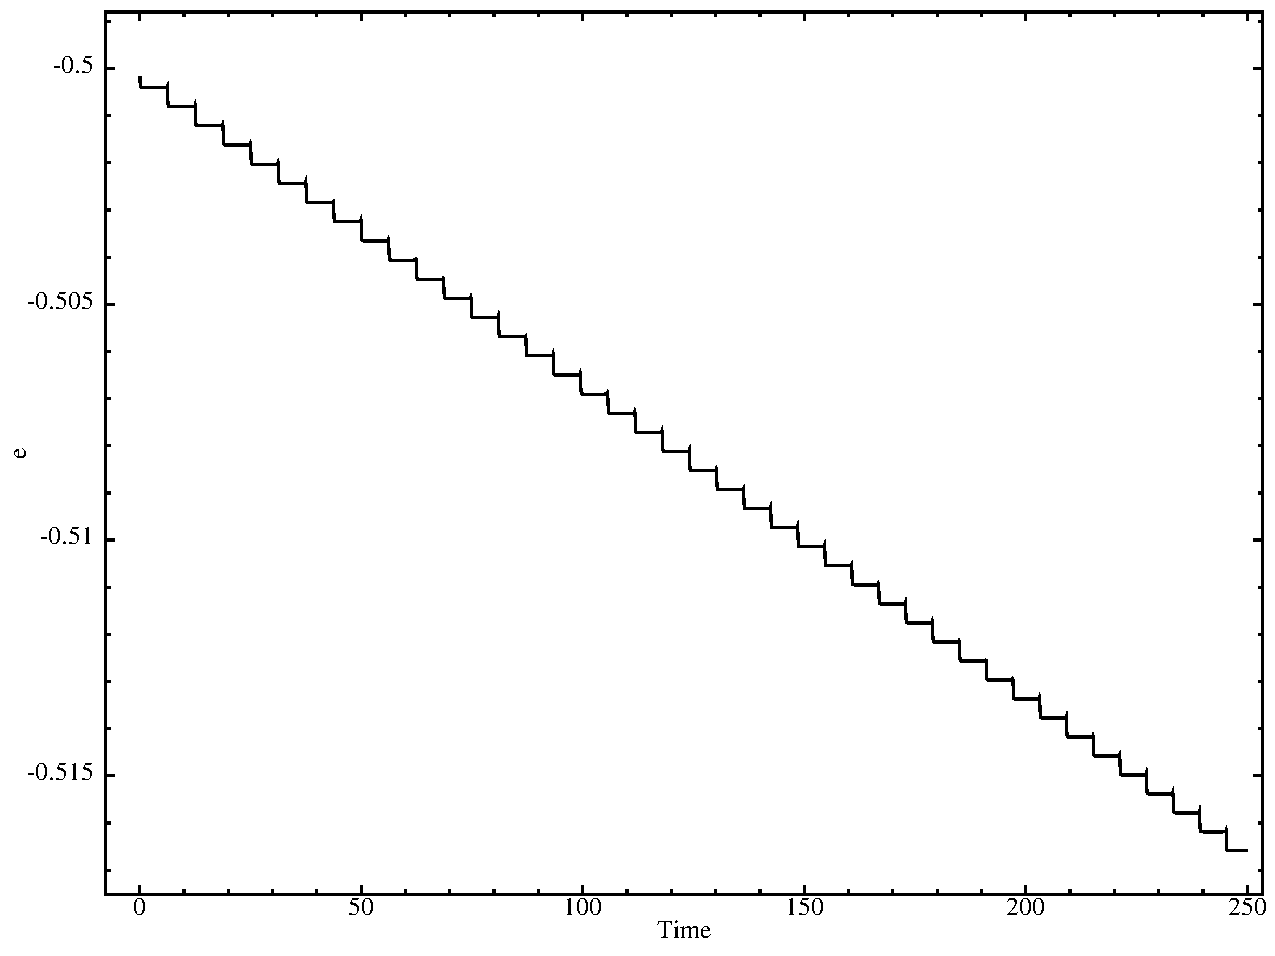
\includegraphics[height=2.2in]{rk40e.pdf}}%
    \caption[]{Angular momentum (top) and total energy (bottom) versus time of
    the orbits using the second order Leapfrog/Velocity Verlet scheme (left) and
    the forth order Runge-Kutta method (right).}.
\end{figure}

\section*{Part 2}
\subsection*{a)}
Figure~\ref{fig:2a} shows the ``1.75D'' magnetised shock at \(t=0.2\). The red
and blue discontinuities correspond to fast and slow waves respectively,
corresponding to the two solutions in the dispersion relation for compressive
waves (\( \mathbf{v\cdot k} \neq 0 \)). Because they are compressive waves, they
are present in every plot. The speed of these waves is given by:

\begin{align}
    v_{wave}^2 &= \frac{\omega^2}{k^2} \\
    &= \frac{1}{2} \left[c_s^2 + v_A^2 \pm \sqrt{(c_s^2 + v_A^2)^2 - 4c_s^2v_a^2 \cos^2 \theta}\right] \, , \label{vwavefs}
    \intertext{But we have} 
    \cos \theta &= \mathbf{\hat{k}} \cdot \frac{ \mathbf{B_0} }{|B_0|} \, \\
    c_s^2 &= \frac{\gamma P^2}{\rho^2} \, \text{, and} \\
    v_A^2 &= \sqrt{B_0^2/(\mu_0 \rho_0)} \, .
    \intertext{For \(x < 0\), and therefore waves travelling to the left, we have:}
    \rho_0 &= 1.08 \, , \\
    P_0 &= 0.95 \, , \\
    \mathbf{B_0} &= (2/ \sqrt{4 \pi },    3.6/ \sqrt{4 \pi}, 2/ \sqrt{4 \pi})^T \, \text{, and}\\
    \mathbf{\hat{k}} &= (-1, 0, 0)^T \\
    \gamma &\approx 1.7
    \intertext{This gives}
    v_{wave} &= 0.39 \, ,
    \intertext{for the slow wave (taking the minus), and}
    v_{wave} &= 1.7 \, ,
    \intertext{for the fast wave. Similarly, For \(x > 0\) (waves travelling to the right), we have:}
    \rho_0 &= 1 \, , \\
    P_0 &= 1 \, , \\
    \mathbf{B_0} &= (2/ \sqrt{4 \pi },    4/ \sqrt{4 \pi}, 2/ \sqrt{4 \pi})^T \, \text{, and}\\
    \mathbf{\hat{k}} &= (1, 0, 0)^T
    \intertext{This gives}
    v_{wave} &= 0.39 \, ,
    \intertext{for the slow wave (taking the minus), and}
    v_{wave} &= 1.8 \, ,
    \intertext{for the fast wave.}
\end{align}

The Alfv\'en waves are not compressive, but can be see in the plots of the
magnetic field and, as well as the velocity in the x and y directions (see
Figure~\ref{fig:2a}). The speed of the Alfv\'en waves can be found from the
dispersion relation as follows:
\begin{align}
    v_{wave}^2 &= \frac{\omega^2}{k^2} \\
    &= v_A^2\cos^2 \theta \, ,. \label{vwavea}
    \intertext{For \(x < 0\), this gives}
    v_{wave} &= 0.54 \, ,
    \intertext{while for \(x > 0\) this gives}
    v_{wave} &= 0.56 \, .
\end{align}
Therefore the speed of the Alfv\'en waves is in between the speed of the slow and
fast waves. This is also reflected on the plots in Figure \ref{fig:2a}.
\begin{figure}[h!]
    \centering
    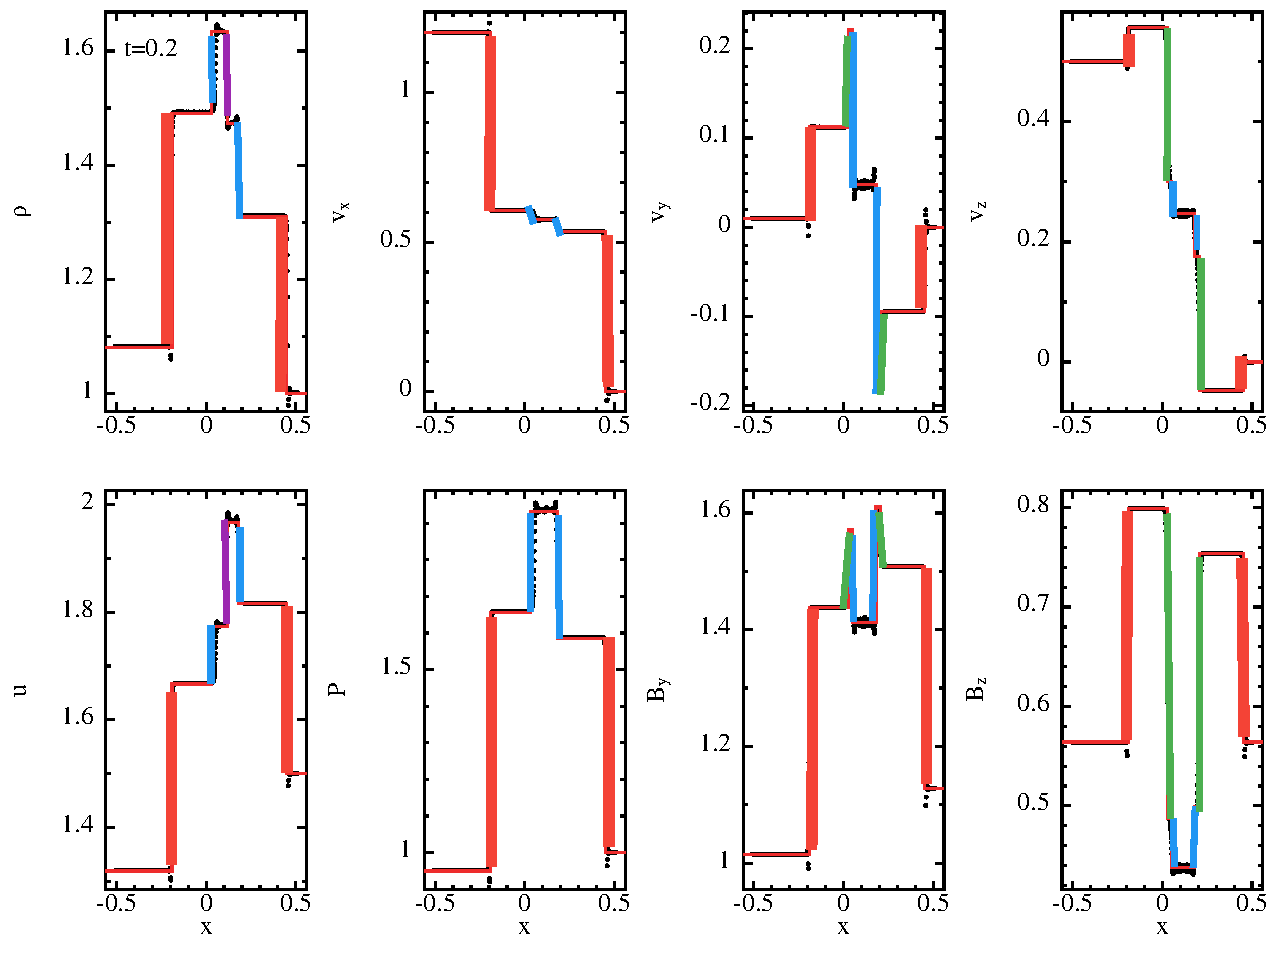
\includegraphics[width=\linewidth]{2a_labeled.pdf}
    \caption{The ``1.75D'' magnetised shock tube. Red Corresponds to a fast wave,
    blue corresponds to a slow wave, green corresponds to an Alfv\'en wave, and
    purple corresponds to a contact discontinuity.
    }
    \label{fig:2a}
\end{figure}

\subsection*{b)}
The initial Alfv\'en speed is given by:
\begin{align}
    v_{A} &= \sqrt{B_0^2/(\mu_0 \rho_0)} \, .
    \intertext{We have:}
    b_0 &= \frac{5}{sqrt{4 \pi}} \, , \\
    \mu_0 &= 1 \, \text{, and}\\
    \rho_0 &= 1 \, ,
    \intertext{giving:}
    v_{A} &\approx 1.4 \, .
    \intertext{Similarly, since we have $\gamma = 1.4$ and $P_0=1$ (see Figure \ref{fig:2b}), we find:}
    c_s &= \sqrt{\frac{\gamma P_0}{\rho_0}}
    &\approx 1.18
    \intertext{For waves traveling in the x direction ($\cos \theta = 1$), Equation \ref{vwavefs} reduces to}
    v_{wave} &= c_s
    \intertext{for slow waves, and}
    v_{wave} &= v_A
    \intertext{for fast waves. In the case of Alfv\'en waves, Equation \ref{vwavea} reduces to}
    v_{wave} &= v_A \, .
    \intertext{Similarly, for waves travelling in the y direction (\cos \theta = 0)}
\end{align} 
The fast waves travel in both the x and y direction, and are slightly faster in
the y direction. These are compressive waves, and are visible in all
the plots.
The slow waves travel mainly in the x direction (they do not travel in the y direction), and are also visible in all plots
as they are also compressive.
The Alfv\'en waves mainly travel in the x direction (the direction of the magnetic
field), and are visible only in the plot showing magnetic energy as they are not
compressive, and so do not show up in either pressure or density.
These are labeled in Figure~\ref{fig:2b}.

\begin{figure}[h!]
    \centering
    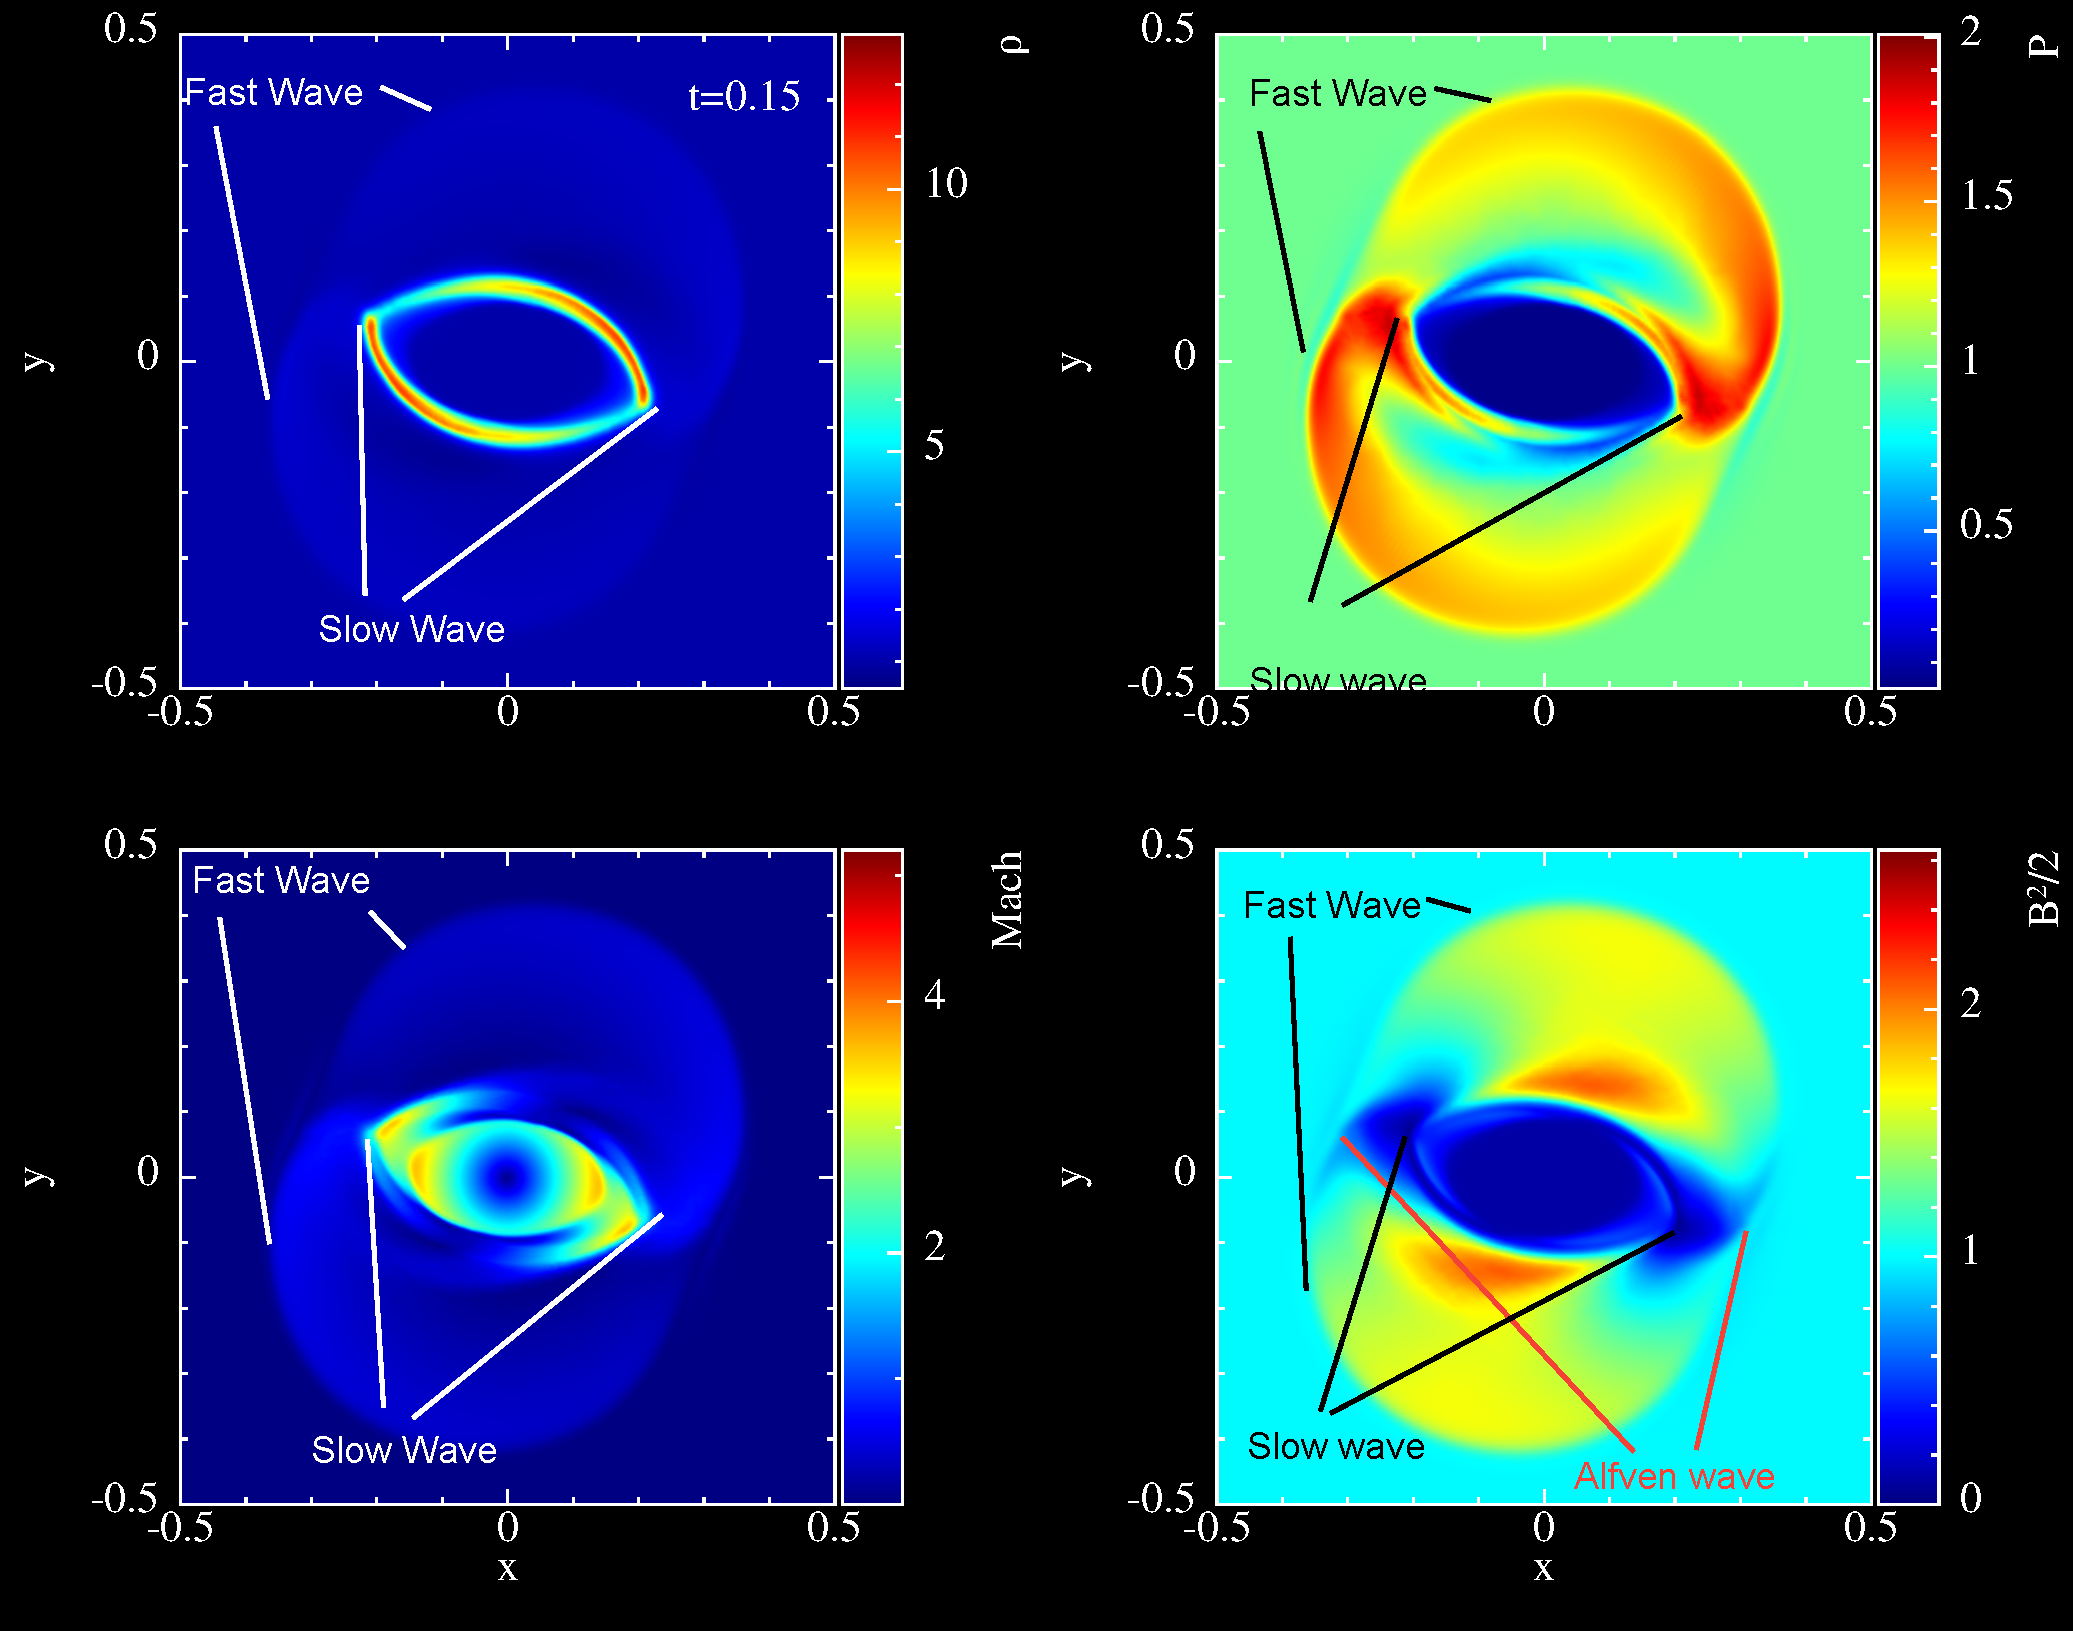
\includegraphics[width=\linewidth]{2b_annotated.pdf}
    \caption{The 2D MHD rotor test, showing the density ($\rho$), pressure
    ($P$), mach number (Mach), and magnetic energy ($B^2/2$). The shockfronts
    for the fast waves, slow waves and Alfv\'en waves are labeled.}
    \label{fig:2b}
\end{figure}

\section*{Part 3}
\subsection*{a)}
The gas and dust velocities after 5 wave periods are show in Figure
\ref{fig:one_fluid} for the one fluid method, and Figure~\ref{fig:two_fluid} for
the two fluid method.
\begin{figure}%
    \centering
    \subfigure[]{%
    \label{fig:one_fluid}%
    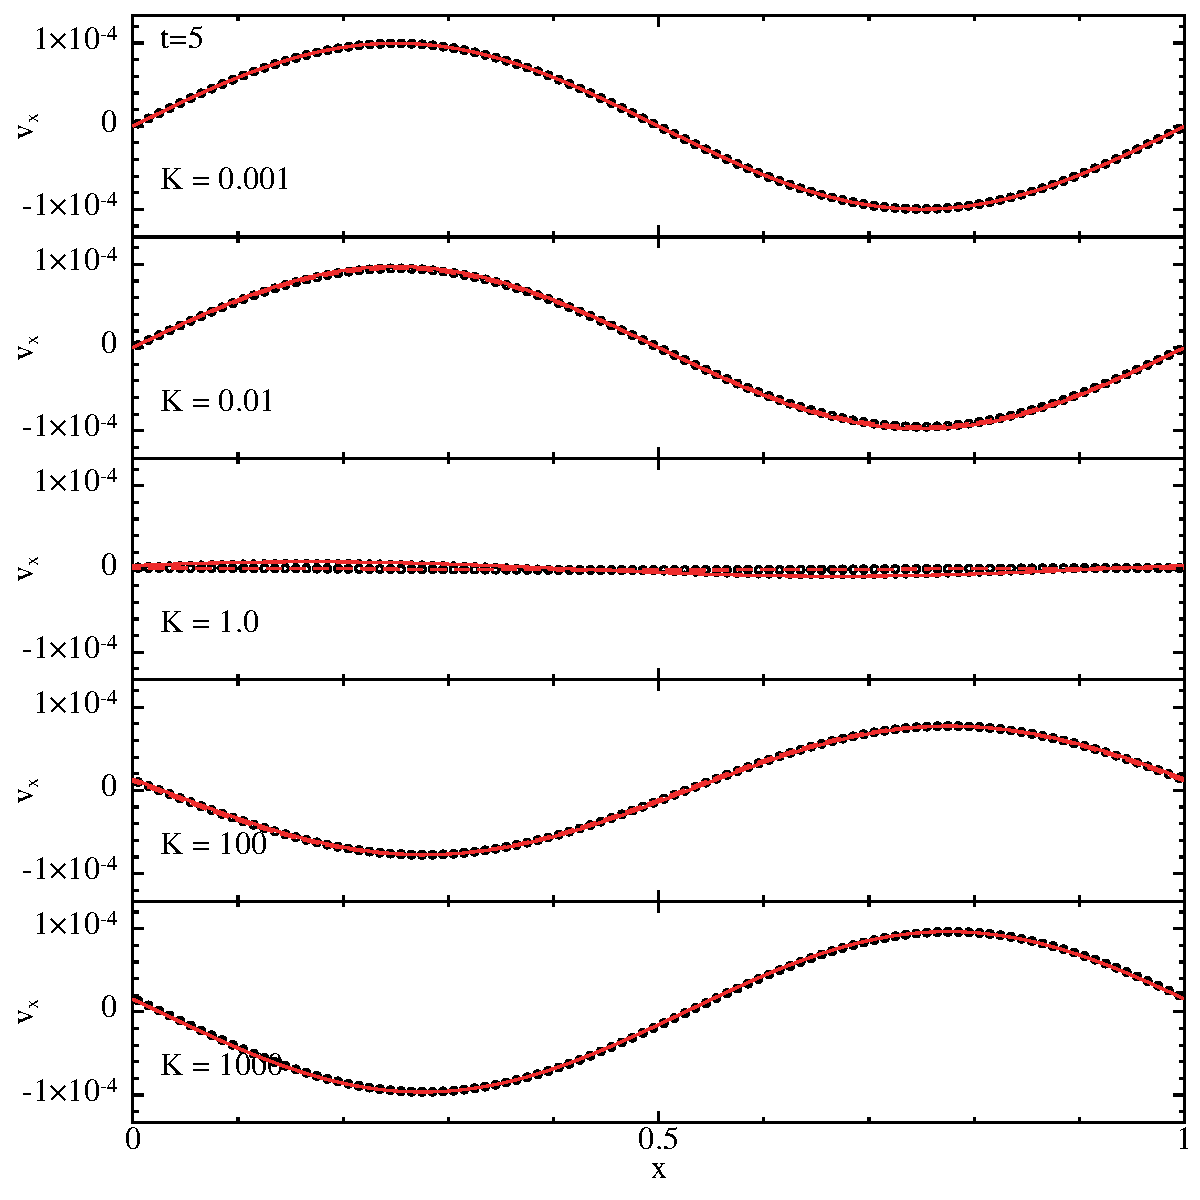
\includegraphics[height=3in]{one_fluid.pdf}}%
    \qquad
    \subfigure[]{%
    \label{fig:two_fluid}%
    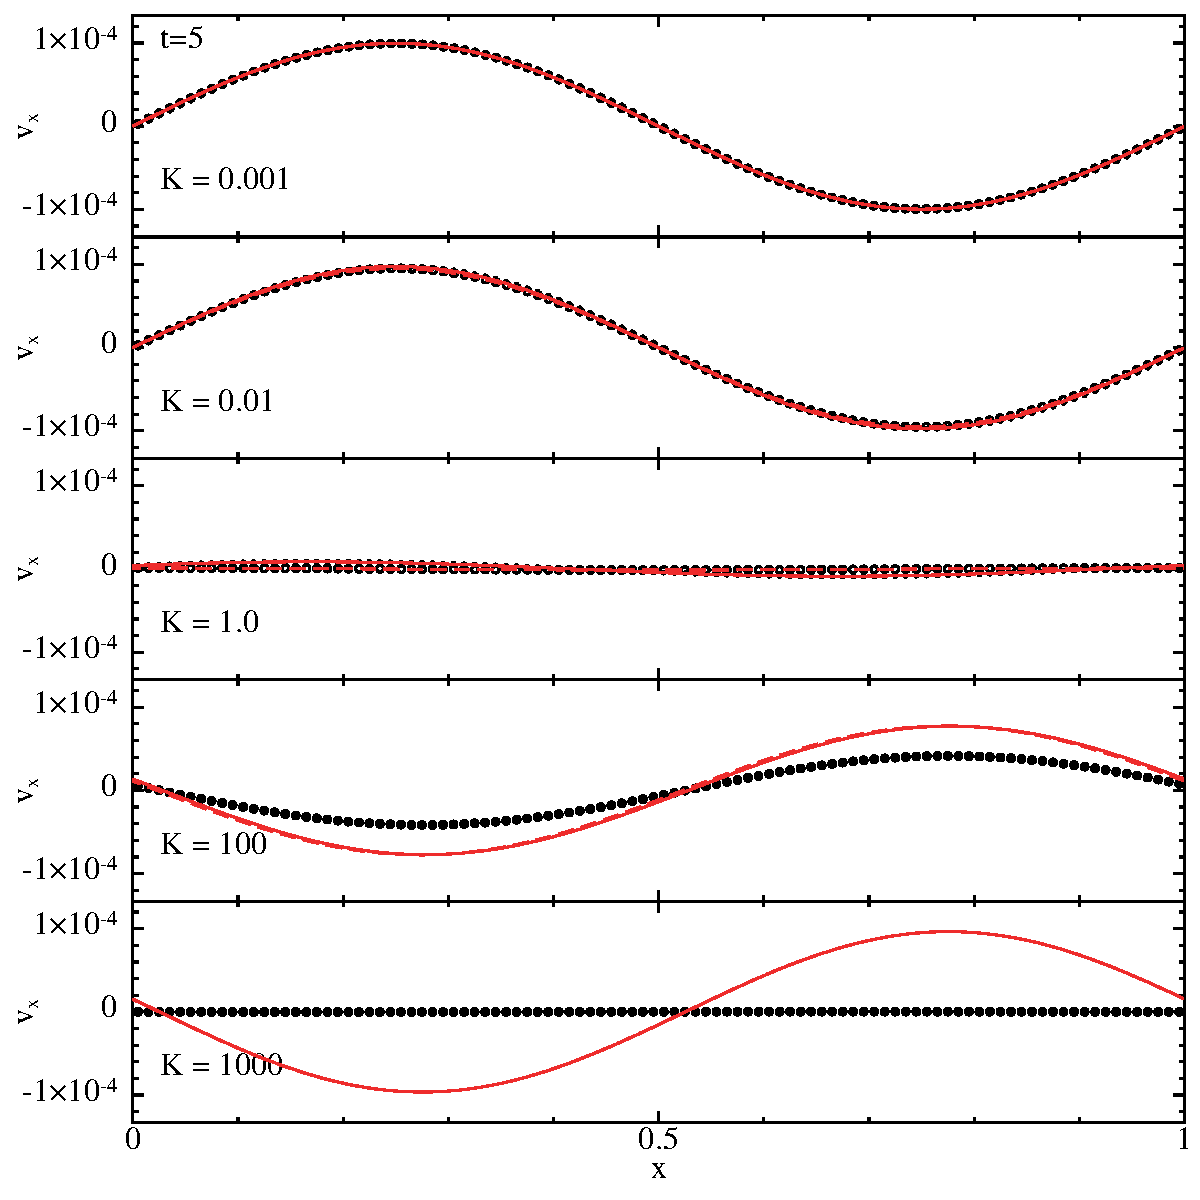
\includegraphics[height=3in]{two_fluid.pdf}}%
    \caption[]{The dusty wave problem for a variety of $K$ values using
    the one fluid method \subref{fig:one_fluid} and the
    two fluid method \subref{fig:two_fluid}.}
    \end{figure}
    
\subsection*{b)}
See end of document

\subsection*{c)}
The stopping time is given by
\begin{align}
    t_s &= \frac{\rho_g \rho_d}{K(\rho_g + \rho_d)} \, .
    \intertext{In our case we have \(\rho_g = \rho_d = 1\), and so we find}
    t_s &= \frac{1}{2K} \, .
\end{align}
We have values of \(K = 0.001, 0.01, 1.0, 100, 1000\), which give stopping times
of \(t_s = 500, 50, 0.5, 0.005, 0.0005\) respectively. For small $K$, (large
stopping time), the dispersion relation reduces to
\begin{align}
    \omega^2 &= k^2 c_s^2 \, ,
    \intertext{while for large $K$, (small stopping time), the dispersion relation reduces to}
    \omega^2 = k^2 \tilde{c}_s^2 \, .
\end{align}

In either case, there is no (or negligible) dampening term, and so the wave
remains undamped, as can be seen in Figures \ref{fig:one_fluid} and
\ref{fig:two_fluid} for both large and small $K$. The only case with dampening
is when $t_s \omega \sim 1 $, i.e. the stopping time is similar to the
timescales involved. This can be seen for the $K = 1.0$ case these figures.


\subsection*{d)}

The two fluid method gives accurate results for small $K$ (i.e. large stopping
times), which occurs when the two fluids are weakly coupled. Assuming Epstein
drag, this corresponds to large grains. As we are dealing with only (small)
linear perturbations, the one fluid method is able to approximate the analytic
solution for all values of $K$ shown in figure \ref{fig:one_fluid}. However for
small $K$ this can break down for non linear perturbations as it is unable to
handle double valued solutions (i.e. dust particles passing through each other)
like the two fluid method. Typically the one fluid method gives the most
accurate results for large K (small stopping times), when the two fluids are
strongly coupled. This corresponds to small grains.

\end{document}
